\documentclass{beamer}

\usepackage{beamerthemesplit}

\setbeamertemplate{footline}[page number]{}

\setbeamertemplate{navigation symbols}{}

\title{Bayes Seminar: Part II}
\author{John Myles White}
\date{\today}

\begin{document}

\frame{\titlepage}

\frame
{
  Automating inference using BUGS:
  \begin{itemize}
    \item{BUGS allows us to build automated systems to perform posterior sampling}
    \item{BUGS constructs a sampler based only on a model description}
    \item{BUGS is a descriptive programming language rather than a procedural programming language}
  \end{itemize}
}

\frame
{
  \begin{itemize}
    \item{A BUGS interpreter works because MCMC sampling is automatable}
    \item{BUGS interpreters often use two types of sampling under the hood:}
    \begin{itemize}
      \item{Gibbs sampling is fully automatable for conjugate parts of models}
      \item{Metropolis-Hasting sampling is automatable even without conjugacy}
    \end{itemize}
  \end{itemize}
}

\frame
{
  Why use BUGS?
  \begin{itemize}
    \item{Separating model descriptions from inference procedures encourages exploration of multiple models}
    \item{Novel models can be built from familiar components without thinking about analytic tractability}
  \end{itemize}
}

\frame
{
  Some BUGS interpreters:
  \begin{itemize}
    \item{WinBUGS}
    \item{OpenBUGS}
    \item{JAGS}
  \end{itemize}
}

\begin{frame}
  \begin{itemize}
    \item{We'll start with inference in the beta-binomial model we used before}
  \end{itemize}
\end{frame}

\begin{frame}[fragile]
  \frametitle{Binomial Model I}

  \begin{verbatim}
model
{
  for (i in 1:N)
  {
    x[i] ~ dbern(p)
  }
  
  p ~ dbeta(alpha, beta)
  
  alpha <- 1
  beta <- 1
}
  \end{verbatim}
\end{frame}

\begin{frame}[fragile]
  \begin{itemize}
    \item{Every BUGS model starts with \verb|model|}
    \item{Primitive looping is allowed}
    \item{Two types of assignment: deterministic and stochastic}
  \end{itemize}
\end{frame}

\begin{frame}[fragile]
  \begin{itemize}
    \item{We've used a beta(1, 1) prior}
    \item{This is a flat prior over $[0, 1]$}
    %\item{VISUALIZE PRIOR}
    %\item{SHOW ALTERNATIVE PRIORS}
  \end{itemize}
\end{frame}

\begin{frame}[fragile]
  \begin{itemize}
    \item{For inference, BUGS needs to be invoked with data}
    \item{We'll use JAGS as our BUGS interpreter}
    \item{We'll use R via the rjags package to send data to JAGS}
    %\item{rjags handles serializing data into the appropriate format for JAGS}
  \end{itemize}
\end{frame}

\begin{frame}[fragile]
  \begin{verbatim}
library('rjags')

df <- read.csv(file.path('data',
                         'binomial',
                         'binomial.csv'))
  \end{verbatim}
\end{frame}

\begin{frame}[fragile]
  For the sample data:
  \begin{itemize}
    \item{$p = 0.4$}
    \item{$n = 5$}
    \item{$\hat{p} = 0.2$}
  \end{itemize}
\end{frame}

\begin{frame}[fragile]
  \begin{verbatim}
"X"
0
0
0
1
0
  \end{verbatim}
\end{frame}

\begin{frame}[fragile]
  \begin{verbatim}
jags <- jags.model(file.path('bugs', 
                             'binomial',
                             'binomial.bugs'),
                   data = list('x' = with(df, X),
                               'N' = nrow(df)),
                   n.chains = 4,
                   n.adapt = 1000)
                   
mcmc.samples <- coda.samples(jags,
                             c('p'),
                             2500)

plot(mcmc.samples)

summary(mcmc.samples)
  \end{verbatim}
\end{frame}

\begin{frame}[fragile]
  \begin{center}
    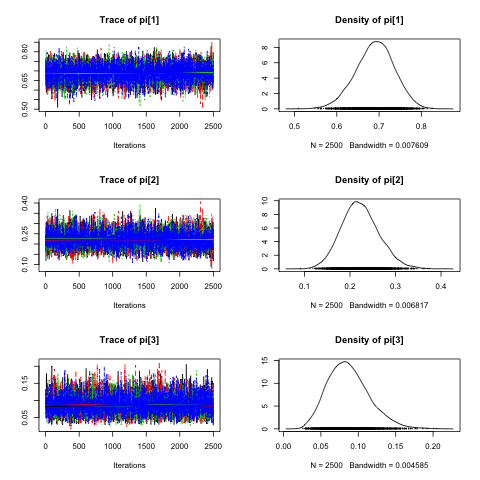
\includegraphics[scale = 0.4]{../JAGSExamples/graphs/binomial/plot.png}
  \end{center}
\end{frame}

\begin{frame}[fragile]
  \begin{verbatim}
Iterations = 1:2500
Thinning interval = 1 
Number of chains = 4 
Sample size per chain = 2500 

1. Empirical mean and standard deviation for each variable,
   plus standard error of the mean:

          Mean             SD       Naive SE Time-series SE 
      0.286161       0.159027       0.001590       0.001576 

2. Quantiles for each variable:

   2.5%     25%     50%     75%   97.5% 
0.04272 0.16242 0.26418 0.39122 0.63907 
  \end{verbatim}
\end{frame}

\begin{frame}[fragile]
  \begin{verbatim}
alpha <- with(df, sum(X) + 1)
beta <- nrow(df) + 2 - alpha

alpha / (alpha + beta)
#[1] 0.2857143

summary(mcmc.samples)$statistics
#          Mean             SD       Naive SE Time-series SE 
#   0.286160728    0.159026669    0.001590267    0.001575952 
  \end{verbatim}
\end{frame}

%\begin{frame}[fragile]
%  \begin{verbatim}
%samples <- data.frame(MCMC = as.matrix(mcmc.samples)[, 1])
%density.plot <- ggplot(samples, aes(x = MCMC)) +
%  geom_density(aes(color = 'Sampling'))
%
%x <- seq(0, 1, by = 0.01)
%analytic <- data.frame(x = x, y = dbeta(x, alpha, beta))
%density.plot <- density.plot +
%  geom_line(data = analytic, aes(x = x,
%                                 y = y,
%                                 color = 'Analytic'))
%  \end{verbatim}
%\end{frame}

\begin{frame}[fragile]
  \begin{center}
    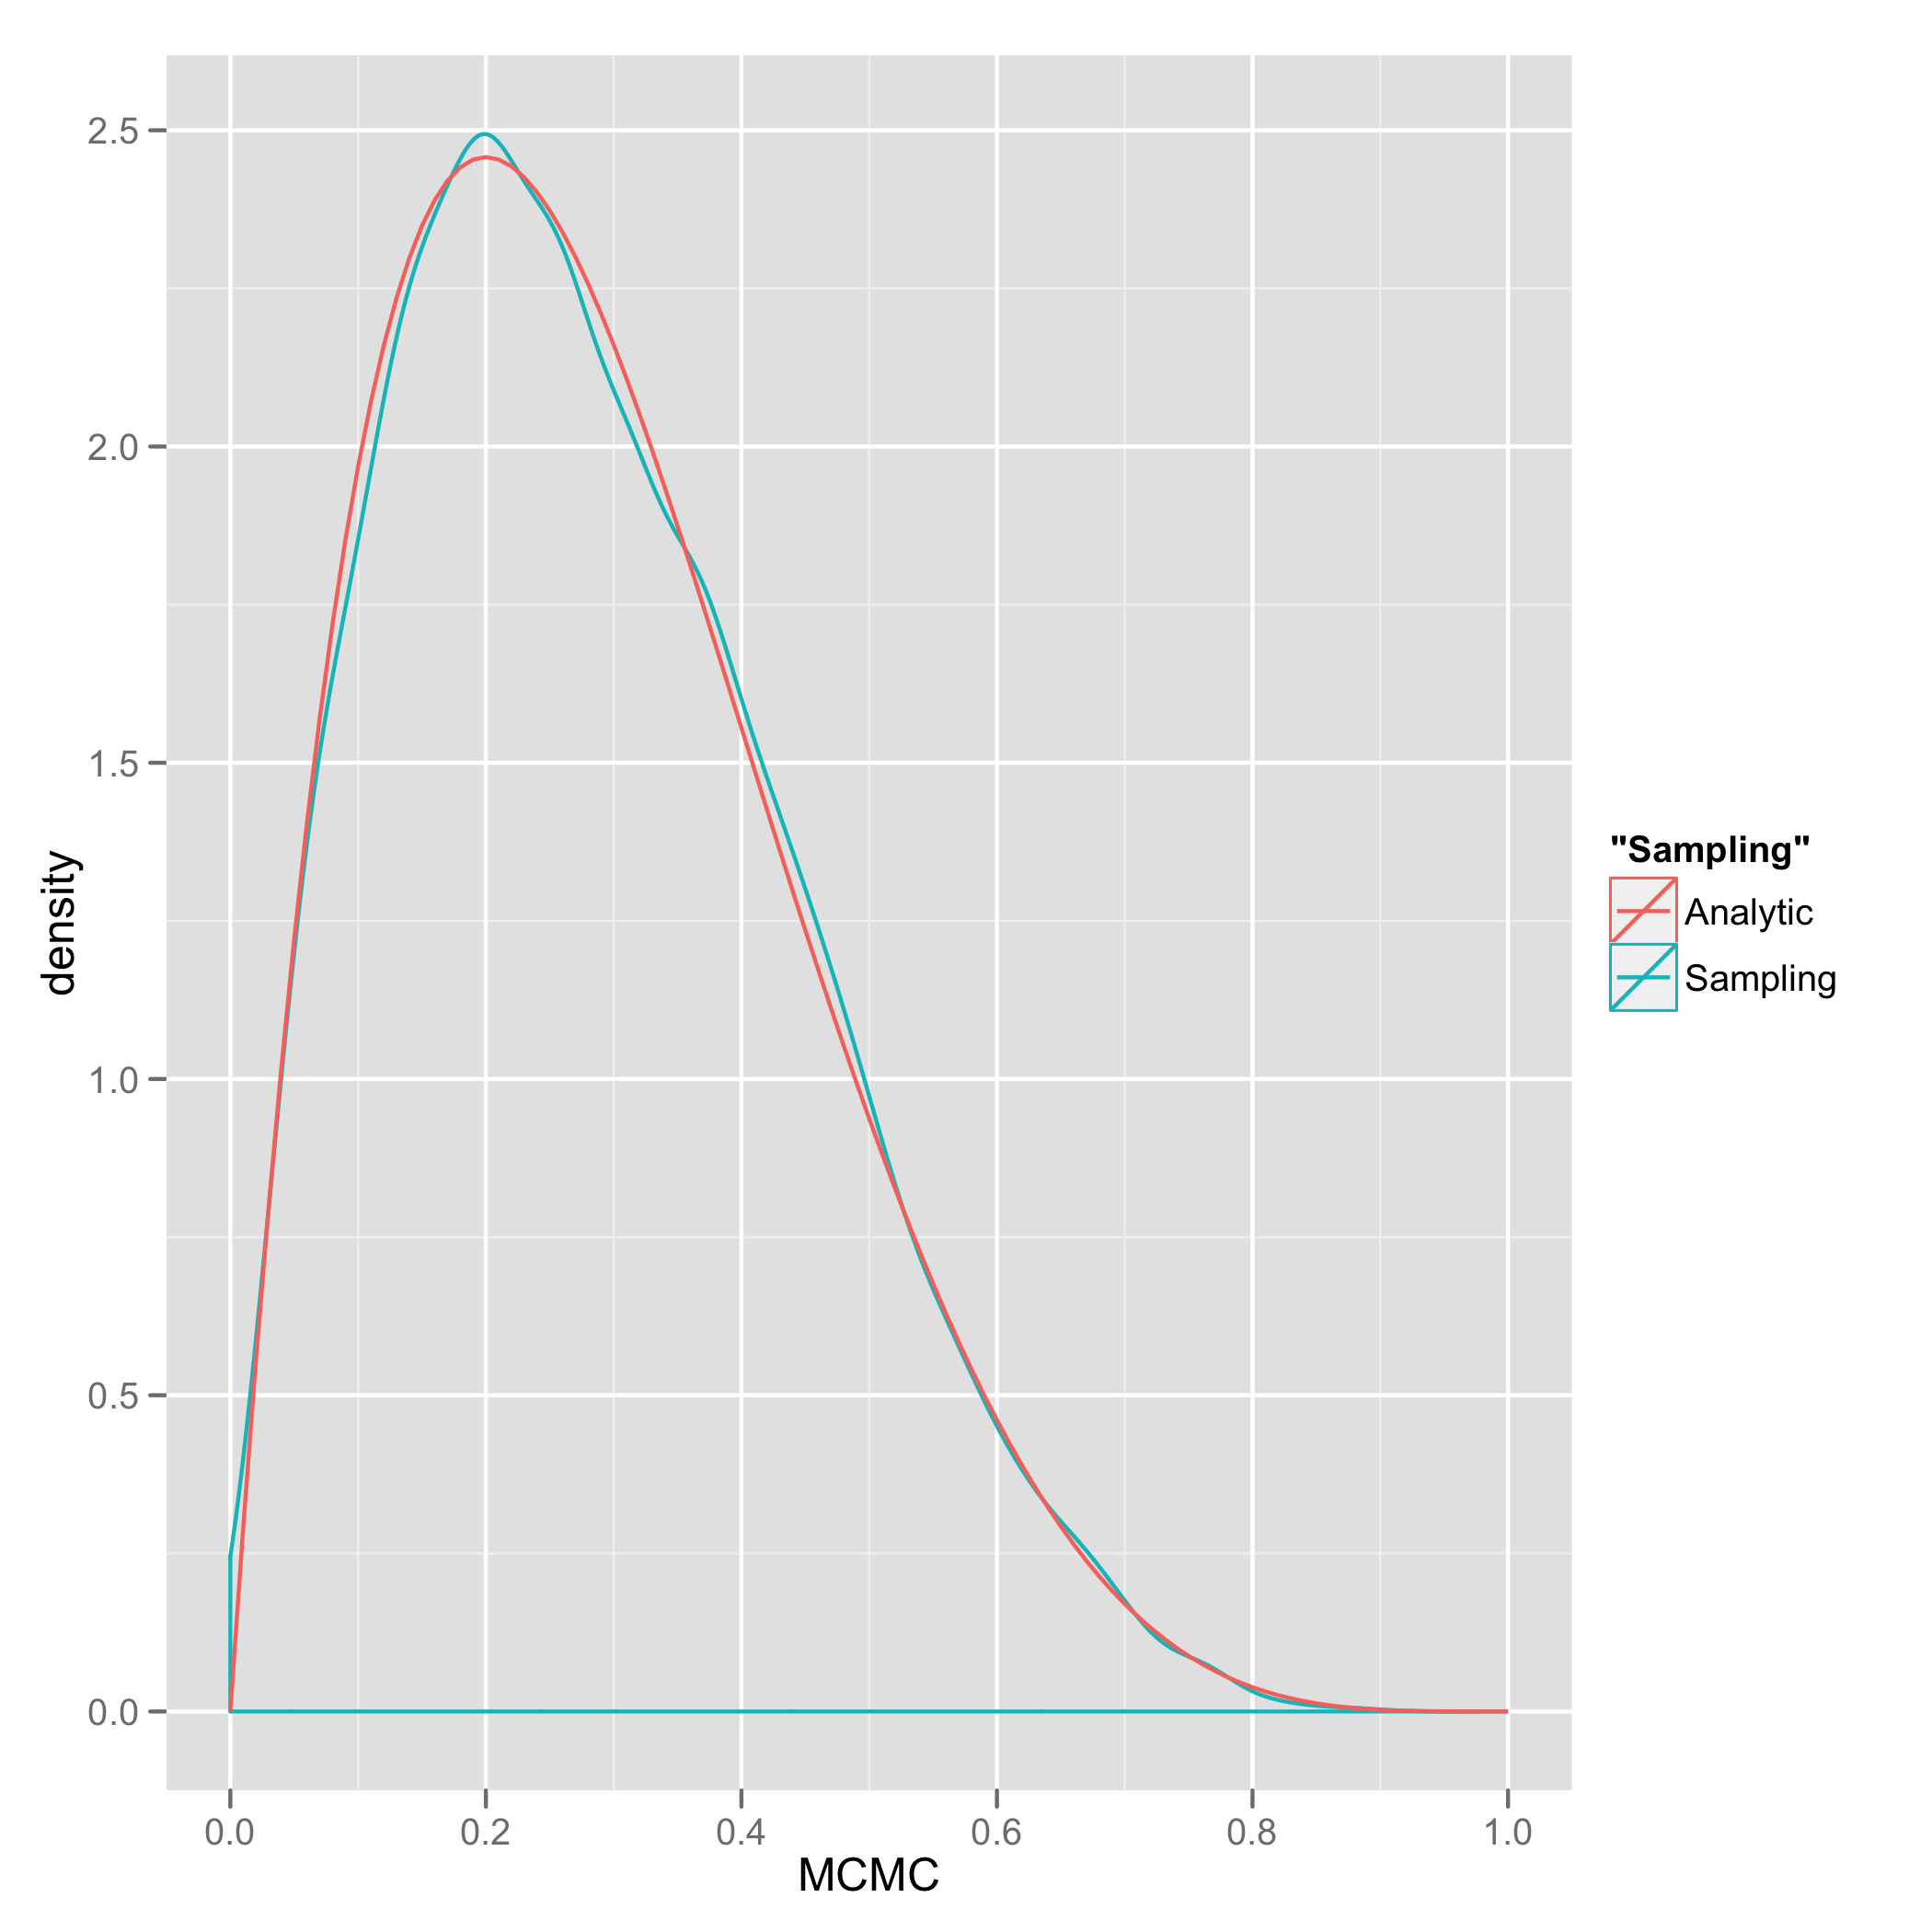
\includegraphics[scale = 0.1]{../JAGSExamples/graphs/binomial/density.png}
  \end{center}
\end{frame}

\begin{frame}[fragile]
  \begin{verbatim}
binom.test(with(df, sum(X)), nrow(df))$conf.int
#[1] 0.005050763 0.716417936
credible.interval <- c(qbeta(0.025, alpha, beta),
                       qbeta(0.975, alpha, beta))
credible.interval
#[1] 0.04327187 0.64123458
binom.test(with(df, sum(X)) + 1, nrow(df) + 2)$conf.int
#[1] 0.03669257 0.70957914
  \end{verbatim}
\end{frame}

\begin{frame}[fragile]
  Lessons:
  
  \begin{itemize}
    \item{BUGS has correctly performed inference}
    \item{Simulation results closely approximate analytic results}
    \item{We get a full posterior, not just a point estimate or CI}
  \end{itemize}
\end{frame}

\begin{frame}[fragile]
  \begin{itemize}
    \item{What could we have done wrong?}
    \item{Used no adaptive phase}
    \item{Gathered too few samples}
  \end{itemize}
\end{frame}

\begin{frame}[fragile]
  \begin{verbatim}
jags <- jags.model(file.path('bugs',
                             'binomial',
                             'binomial.bugs'),
                   data = list('x' = with(df, X),
                               'N' = nrow(df)),
                   n.chains = 4,
                   n.adapt = 0)
                   
mcmc.samples <- coda.samples(jags,
                             c('p'),
                             100)

plot(mcmc.samples)
  \end{verbatim}
\end{frame}

\begin{frame}[fragile]
  \begin{center}
    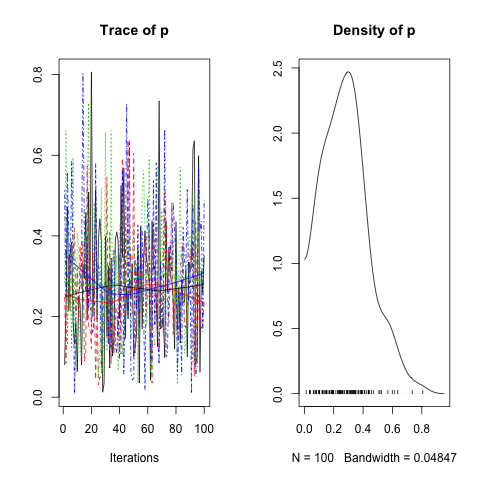
\includegraphics[scale = 0.4]{../JAGSExamples/graphs/binomial/broken_plot.png}
  \end{center}
\end{frame}

\begin{frame}[fragile]
  \begin{itemize}
    \item{You should play with this example more and try to break it}
    \item{In this case, having no adaptive phase turns out not to matter}
    \item{Using too few samples gives us a wiggly approximation to the posterior}
  \end{itemize}
\end{frame}

\begin{frame}[fragile]
  \begin{itemize}
    \item{Let's move on to inferring the mean of a normal distribution}
  \end{itemize}
\end{frame}

\begin{frame}[fragile]
  \begin{verbatim}
model
{
  for (i in 1:N)
  {
    x[i] ~ dnorm(mu, tau)
  }
  
  mu ~ dnorm(0, 0.0001)
  
  sigma <- 3
  tau <- pow(sigma, -2)
}
  \end{verbatim}
\end{frame}

\begin{frame}[fragile]
  \begin{itemize}
    \item{BUGS uses precision rather than variance to specify normal distributions}
    \item{We use a weakly informative Normal prior centered at zero}
    \item{We use arithmetic within BUGS to transform variance into precision}
  \end{itemize}
\end{frame}

\begin{frame}[fragile]
  For sample data:
  \begin{itemize}
    \item{$\mu = 25$}
    \item{$\sigma = 3$}
    \item{$n = 100$}
    \item{$\hat{\mu} = 25.32666$}
  \end{itemize}
\end{frame}

\begin{frame}[fragile]
  \begin{verbatim}
"X"
23.120638567773
25.5509299726662
22.4931141627699
...
23.2802037572893
21.3261621553049
23.5797980906821
  \end{verbatim}
\end{frame}


\begin{frame}[fragile]
  \begin{verbatim}
library('rjags')

df <- read.csv(file.path('data',
                         'normal',
                         'normal_mean.csv'))
  \end{verbatim}
\end{frame}

\begin{frame}[fragile]
  \begin{verbatim}
jags <- jags.model(file.path('bugs',
                             'normal',
                             'normal_mean.bugs'),
                   data = list('x' = with(df, X),
                               'N' = nrow(df)),
                   n.chains = 4,
                   n.adapt = 500)
                   
mcmc.samples <- coda.samples(jags,
                             c('mu'),
                             1000)

plot(mcmc.samples)

summary(mcmc.samples)
  \end{verbatim}
\end{frame}

\begin{frame}[fragile]
  \begin{verbatim}
Iterations = 1:1000
Thinning interval = 1 
Number of chains = 4 
Sample size per chain = 1000 

1. Empirical mean and standard deviation for each variable,
   plus standard error of the mean:

          Mean             SD       Naive SE Time-series SE 
     25.331926       0.303623       0.004801       0.004849 

2. Quantiles for each variable:

 2.5%   25%   50%   75% 97.5% 
24.74 25.13 25.32 25.53 25.93 
  \end{verbatim}
\end{frame}

\begin{frame}[fragile]
  \begin{center}
    \includegraphics[scale = 0.4]{../JAGSExamples/graphs/normal/plot1.png}
  \end{center}
\end{frame}

%\begin{frame}[fragile]
%Frequentist CI
%Credible interval
%\end{frame}

\begin{frame}[fragile]
  \begin{itemize}
    \item{As in the binomial example, we have a conjugate prior here}
    \item{Posterior has closed form solution, which could be used to assess quality of MCMC}
    \item{But we see that MCMC solution is the MLE so we skip that analysis}
  \end{itemize}
\end{frame}

\begin{frame}[fragile]
  \begin{itemize}
    \item{Let's show that inference can be very bad if the wrong prior is used}
  \end{itemize}
\end{frame}

\begin{frame}[fragile]
  \begin{verbatim}
model
{
  for (i in 1:N)
  {
    x[i] ~ dnorm(mu, tau)
  }
  
  mu ~ dnorm(0, 10)
  
  sigma <- 3
  tau <- pow(sigma, -2)
}
  \end{verbatim}
\end{frame}

\begin{frame}[fragile]
  \begin{itemize}
    \item{Prior has mean $0$}
    \item{Prior has variance $\frac{1}{10}$}
    \item{With so little variance, the prior pulls the posterior towards itself}
  \end{itemize}
\end{frame}

\begin{frame}[fragile]
  \begin{verbatim}
Iterations = 1:1000
Thinning interval = 1 
Number of chains = 4 
Sample size per chain = 1000 

1. Empirical mean and standard deviation for each variable,
   plus standard error of the mean:

          Mean             SD       Naive SE Time-series SE 
     13.327539       0.215767       0.003412       0.003343 

2. Quantiles for each variable:

 2.5%   25%   50%   75% 97.5% 
12.92 13.18 13.32 13.47 13.75 
  \end{verbatim}
\end{frame}

\begin{frame}[fragile]
  \begin{center}
    \includegraphics[scale = 0.4]{../JAGSExamples/graphs/normal/plot2.png}
  \end{center}
\end{frame}

\begin{frame}
  \begin{itemize}
    \item{It can easily get worse}
  \end{itemize}
\end{frame}

\begin{frame}[fragile]
  \begin{verbatim}
model
{
  for (i in 1:N)
  {
    x[i] ~ dnorm(mu, tau)
  }
  
  mu ~ dnorm(-1000, 10)
  
  sigma <- 3
  tau <- pow(sigma, -2)
}
  \end{verbatim}
\end{frame}

\begin{frame}[fragile]
  \begin{verbatim}
Iterations = 1:1000
Thinning interval = 1 
Number of chains = 4 
Sample size per chain = 1000 

1. Empirical mean and standard deviation for each variable,
   plus standard error of the mean:

          Mean             SD       Naive SE Time-series SE 
    -4.604e+02      2.164e-01      3.422e-03      3.507e-03 

2. Quantiles for each variable:

  2.5%    25%    50%    75%  97.5% 
-460.8 -460.5 -460.4 -460.2 -459.9 
  \end{verbatim}
\end{frame}

\begin{frame}[fragile]
  \begin{center}
    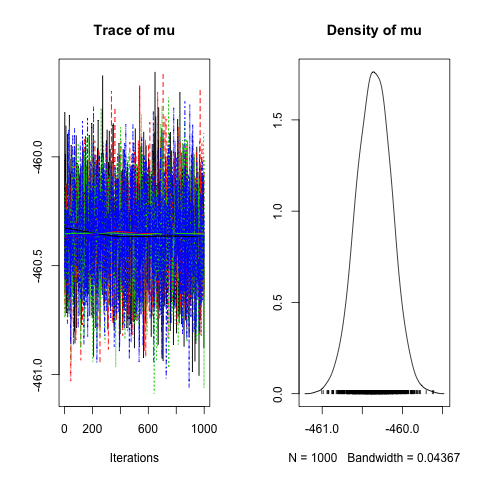
\includegraphics[scale = 0.4]{../JAGSExamples/graphs/normal/plot3.png}
  \end{center}
\end{frame}

\begin{frame}[fragile]
  \begin{itemize}
    \item{Using the wrong prior variance causes trouble}
    \item{Using the wrong prior mean causes more trouble}
    \item{Using the wrong prior functional form can be still worse}
  \end{itemize}
\end{frame}

\begin{frame}[fragile]
  \begin{verbatim}
model
{
  for (i in 1:N)
  {
    x[i] ~ dnorm(mu, tau)
  }
  
  mu ~ dunif(0, 1)
  
  sigma <- 3
  tau <- pow(sigma, -2)
}
  \end{verbatim}
\end{frame}

\begin{frame}[fragile]
  \begin{center}
    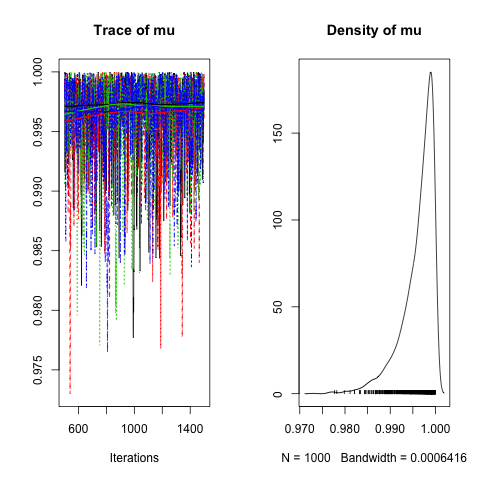
\includegraphics[scale = 0.4]{../JAGSExamples/graphs/normal/plot4.png}
  \end{center}
\end{frame}

\begin{frame}[fragile]
  \begin{verbatim}
Iterations = 501:1500
Thinning interval = 1 
Number of chains = 4 
Sample size per chain = 1000 

1. Empirical mean and standard deviation for each variable,
   plus standard error of the mean:

          Mean             SD       Naive SE Time-series SE 
     9.962e-01      3.691e-03      5.836e-05      1.361e-04 

2. Quantiles for each variable:

  2.5%    25%    50%    75%  97.5% 
0.9861 0.9946 0.9973 0.9989 0.9999 
  \end{verbatim}
\end{frame}

\begin{frame}[fragile]
  \begin{itemize}
    \item{Because our prior assigns 0 probability to most values of $\mu$, it can't reach them even with infinite data}
    \item{Lindley refers to the requirement that priors not assign 0 probability as Cromwell's Rule:}
  \begin{quote}
I beseech you, in the bowels of Christ, think it possible that you may be mistaken.
  \end{quote}
  \item{When you violate Cromwell's Rule, you can get extremely tight posteriors around very wrong values}
  \item{In this case, you can discover your mistake because of the truncated posterior}
  \end{itemize}
\end{frame}

\begin{frame}[fragile]
  \begin{itemize}
    \item{But take away this lesson:}
    \begin{itemize}
      \item{If you have valid prior information, put it in the prior}
      \item{Otherwise, give the prior very high variance}
    \end{itemize}
  \end{itemize}
\end{frame}

% Normal mean and variance inference (uniform prior)
% Normal mean and variance inference (gamma prior)

\begin{frame}[fragile]
  \begin{itemize}
    \item{Let's leave single parameter inference behind}
    \item{We'll implement a Bayesian linear regression}
  \end{itemize}
\end{frame}

\begin{frame}[fragile]
  \begin{verbatim}
model
{
  for (i in 1:N)
  {
    y[i] ~ dnorm(mu[i], tau)
    mu[i] <- a * x[i] + b
  }
  
  a ~ dnorm(0, 0.0001)
  b ~ dnorm(0, 0.0001)
  
  tau <- pow(sigma, -2)
  sigma ~ dunif(0, 10000)
}
  \end{verbatim}
\end{frame}

\begin{frame}[fragile]
  \begin{verbatim}
"X","Y"
0,84.3386547314417
0.1,105.591083105552
0.2,81.1092846897488
0.3,142.882020053445
...
9.7,182.668364644078
9.8,167.384684627541
9.9,187.164984089017
10,184.490833069397
  \end{verbatim}
\end{frame}

\begin{frame}
  For the sample data:
  \begin{itemize}
    \item{$a = 10$}
    \item{$b = 100$}
    \item{$\sigma = 25$}
  \end{itemize}
\end{frame}

\begin{frame}[fragile]
  \begin{verbatim}
library('rjags')

df <- read.csv(file.path('data',
                         'ols',
                         'ols_regression.csv'))

with(df, plot(X, Y))
  \end{verbatim}
\end{frame}

\begin{frame}[fragile]
  \begin{center}
    \includegraphics[scale = 0.4]{../JAGSExamples/graphs/ols/data_plot.png}
  \end{center}
\end{frame}

\begin{frame}[fragile]
  \begin{verbatim}
jags <- jags.model(file.path('bugs',
                             'ols',
                             'ols_regression.bugs'),
                   data = list('x' = with(df, X),
                               'y' = with(df, Y),
                               'N' = nrow(df)),
                   n.chains = 4,
                   n.adapt = 1000)
 
mcmc.samples <- coda.samples(jags,
                        c('a', 'b', 'sigma'),
                        1000)

plot(mcmc.samples)

summary(mcmc.samples)
  \end{verbatim}
\end{frame}

\begin{frame}[fragile]
  \begin{center}
    \includegraphics[scale = 0.4]{../JAGSExamples/graphs/ols/plot1.png}
  \end{center}
\end{frame}

\begin{frame}[fragile]
  \begin{verbatim}
Iterations = 1001:2000
Thinning interval = 1 
Number of chains = 4 
Sample size per chain = 1000 

1. Empirical mean and standard deviation for each variable,
   plus standard error of the mean:

         Mean     SD Naive SE Time-series SE
a       9.875 0.8035  0.01270        0.03743
b     103.023 4.6591  0.07367        0.22097
sigma  22.805 1.6429  0.02598        0.03003

2. Quantiles for each variable:

        2.5%     25%     50%    75%  97.5%
a      8.239   9.349   9.887  10.40  11.45
b     93.962  99.996 103.088 105.97 112.60
sigma 19.895  21.640  22.687  23.83  26.32
  \end{verbatim}
\end{frame}

\begin{frame}[fragile]
  \begin{verbatim}
Call:
lm(formula = Y ~ X, data = df)

Coefficients:
(Intercept)            X  
    103.620        9.784  
  \end{verbatim}
\end{frame}

\begin{frame}[fragile]
  \begin{itemize}
    \item{Implementing simple linear regression is easy}
    \item{BUGS's virtue is that alternatives are just as easy to implement}
  \end{itemize}
\end{frame}

\begin{frame}[fragile]
  \begin{itemize}
    \item{Consider a case where the Gaussian noise assumption is wrong}
    \item{One solution is to replace the OLS objective with the LAD objective}
    \item{For a Bayesian this amounts to assuming Laplace noise}
  \end{itemize}
\end{frame}

\begin{frame}[fragile]
  \begin{verbatim}
library('rjags')

df <- read.csv(file.path('data',
                         'ols',
                         'ols_regression_outlier.csv'))

with(df, plot(X, Y))
  \end{verbatim}
\end{frame}

\begin{frame}[fragile]
  \begin{center}
    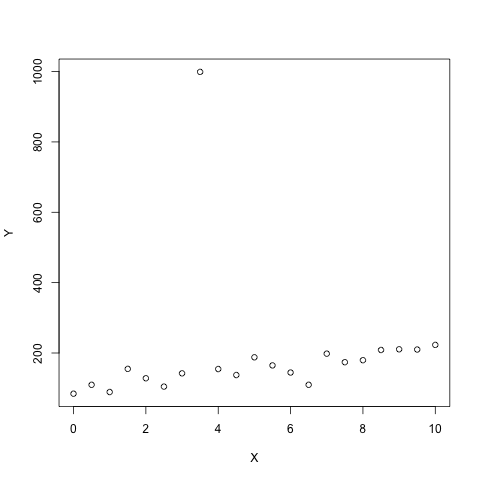
\includegraphics[scale = 0.4]{../JAGSExamples/graphs/ols/outlier_data_plot.png}
  \end{center}
\end{frame}

\begin{frame}
  For the sample data:
  \begin{itemize}
    \item{$a = 10$}
    \item{$b = 100$}
    \item{$\sigma = 25$}
    \item{One outlier was added post hoc}
  \end{itemize}
\end{frame}

\begin{frame}[fragile]
  \begin{verbatim}
jags <- jags.model(file.path('bugs',
                             'ols',
                             'ols_regression_outlier.bugs'),
                   data = list('x' = with(df, X),
                               'y' = with(df, Y),
                               'N' = nrow(df)),
                   n.chains = 4,
                   n.adapt = 1000)
 
mcmc.samples <- coda.samples(jags,
                        c('a', 'b', 'sigma'),
                        5000)

plot(mcmc.samples)

summary(mcmc.samples)
  \end{verbatim}
\end{frame}

\begin{frame}[fragile]
  \begin{center}
    \includegraphics[scale = 0.4]{../JAGSExamples/graphs/ols/plot2.png}
  \end{center}
\end{frame}

\begin{frame}[fragile]
  \begin{verbatim}
Iterations = 1001:6000
Thinning interval = 1 
Number of chains = 4 
Sample size per chain = 5000 

1. Empirical mean and standard deviation for each variable,
   plus standard error of the mean:

        Mean    SD Naive SE Time-series SE
a      15.41 12.27  0.08675         0.1764
b      98.72 65.88  0.46585         0.9934
sigma 208.10 36.85  0.26056         0.4147

2. Quantiles for each variable:

         2.5%     25%    50%    75%  97.5%
a      -8.068   7.127  15.16  23.55  39.64
b     -33.903  54.731  99.57 143.41 225.82
sigma 150.876 181.921 203.17 228.62 293.77
  \end{verbatim}
\end{frame}

\frame
{
  \begin{itemize}
    \item{Using a heavier-tailed error distribution gives the outlier less influence}
    \item{We use Laplace errors, but we could other distributions}
  \end{itemize}
}

\begin{frame}[fragile]
  \begin{verbatim}
model
{
  for (i in 1:N)
  {
    y[i] ~ ddexp(mu[i], tau)
    mu[i] <- a * x[i] + b
  }
  
  a ~ dnorm(0, 0.0001)
  b ~ dnorm(0, 0.0001)
  
  tau <- pow(sigma, -2)
  sigma ~ dunif(0, 100)
}

  \end{verbatim}
\end{frame}

\begin{frame}[fragile]
  \begin{verbatim}
library('rjags')

df <- read.csv(file.path('data',
                         'lad',
                         'lad_regression.csv'))

with(df, plot(X, Y))
  \end{verbatim}
\end{frame}

\begin{frame}[fragile]
  \begin{verbatim}
jags <- jags.model(file.path('bugs',
                             'lad',
                             'lad_regression.bugs'),
                   data = list('x' = with(df, X),
                               'y' = with(df, Y),
                               'N' = nrow(df)),
                   n.chains = 4,
                   n.adapt = 1000)
 
mcmc.samples <- coda.samples(jags,
                        c('a', 'b', 'sigma'),
                        1000)

plot(mcmc.samples)

summary(mcmc.samples)
  \end{verbatim}
\end{frame}

\begin{frame}[fragile]
  \begin{center}
    \includegraphics[scale = 0.4]{../JAGSExamples/graphs/lad/plot1.png}
  \end{center}
\end{frame}

\begin{frame}[fragile]
  \begin{verbatim}
Iterations = 1001:2000
Thinning interval = 1 
Number of chains = 4 
Sample size per chain = 1000 

1. Empirical mean and standard deviation for each variable,
   plus standard error of the mean:

        Mean      SD Naive SE Time-series SE
a     11.956  3.1146  0.04925        0.18855
b     97.419 19.0487  0.30119        1.10237
sigma  7.959  0.9604  0.01519        0.02498

2. Quantiles for each variable:

        2.5%    25%    50%     75%  97.5%
a      5.654 10.144 12.038  13.811  18.28
b     59.353 85.228 98.091 108.933 135.82
sigma  6.361  7.264  7.869   8.513  10.22
  \end{verbatim}
\end{frame}

\frame
{
  \begin{itemize}
    \item{Our inferences for $a$ and $b$ are much better}
    \item{$\sigma$ is no longer meaningful since we have a different error distribution}
  \end{itemize}
}

\begin{frame}
  \begin{itemize}
    \item{Visualizing the OLS and LAD lines is even more compelling}
  \end{itemize}
\end{frame}

%\begin{frame}[fragile]
%  \begin{verbatim}
%lad.coef <- summary(mcmc.samples)$statistics[c(2, 1), 1]
%ols.coef <- coef(lm(Y ~ X, data = df))
%
%library('ggplot2')
%
%ggplot(df, aes(x = X, y = Y)) +
%  geom_point() +
%  geom_abline(intercept = lad.coef[1],
%              slope = lad.coef[2],
%              color = "blue") +
%  geom_abline(intercept = ols.coef[1],
%              slope = ols.coef[2],
%              color = "green")
%  \end{verbatim}
%\end{frame}

\begin{frame}[fragile]
  \begin{center}
    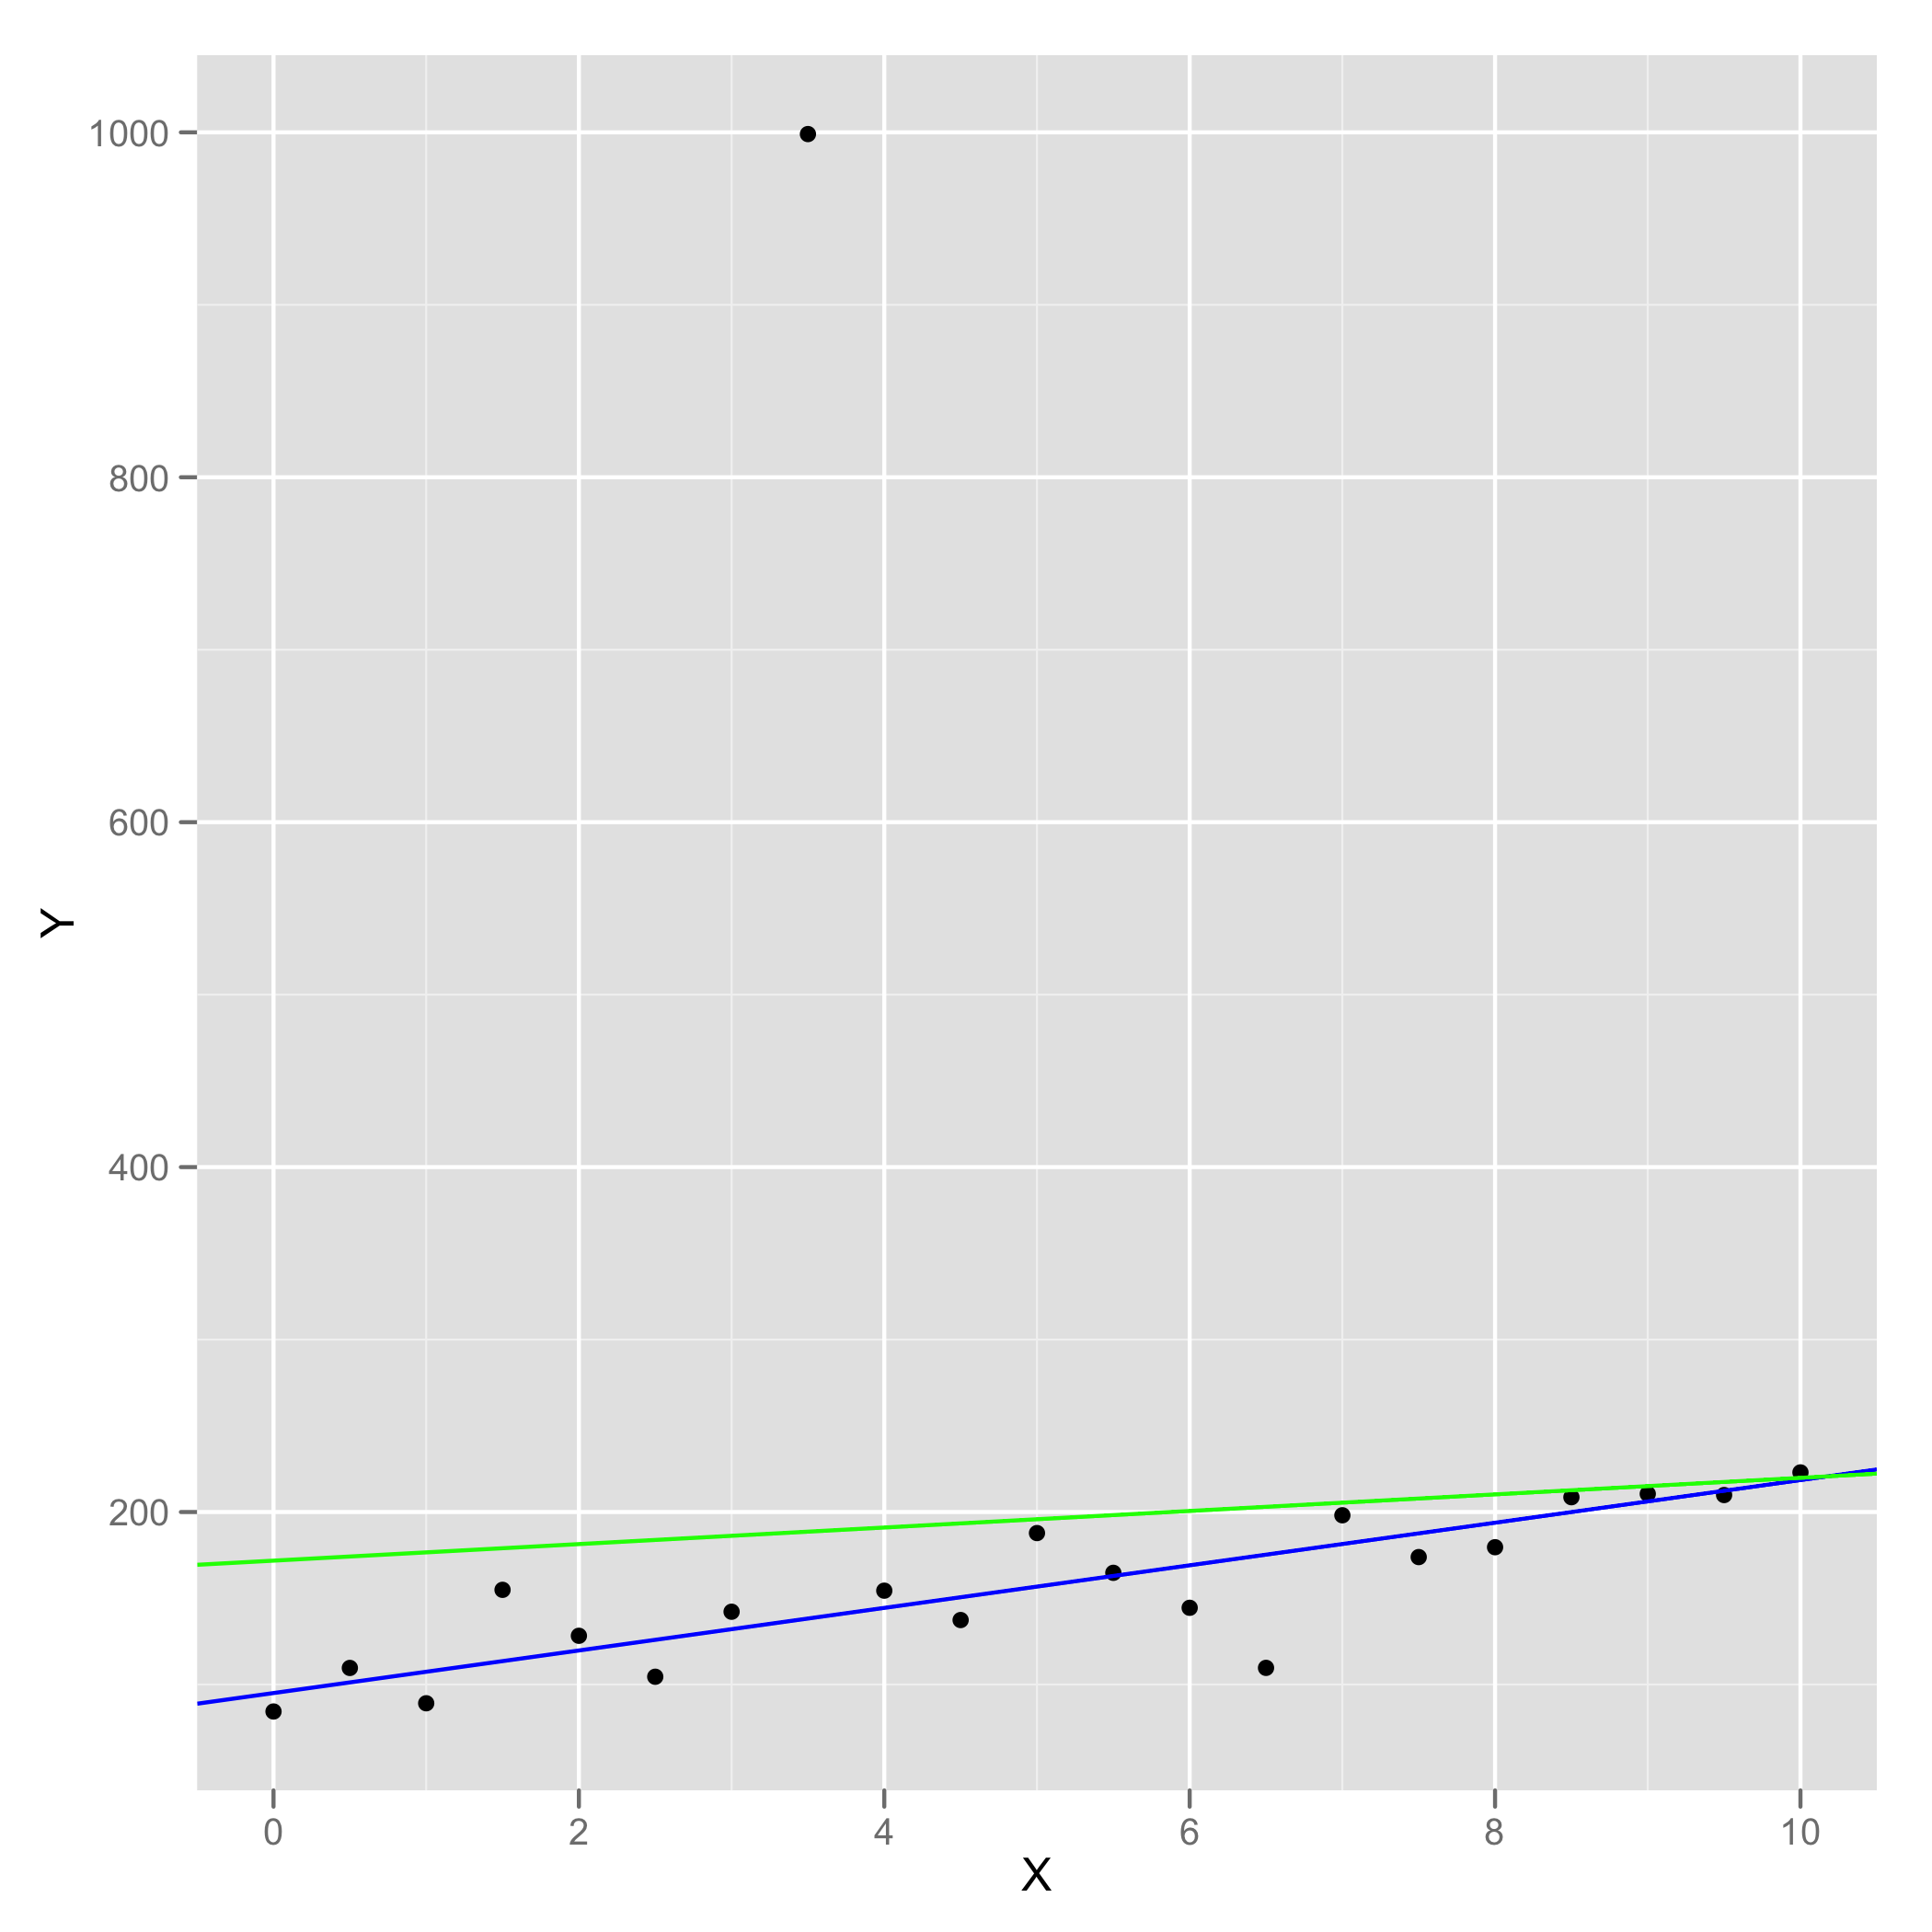
\includegraphics[scale = 0.1]{../JAGSExamples/graphs/lad/lad_vs_ols.png}
  \end{center}
\end{frame}

%\begin{frame}[fragile]
%  \begin{itemize}
%    \item{Our OLS and LAD models are technically not the OLS and LAD solutions}
%    \item{Because we did not use flat priors, our models are closed to ridge regression}
%    \item{By changing our coefficient priors, we can produce the Bayesian equivalent of the Lasso}
%  \end{itemize}
%\end{frame}

%\begin{frame}
%LASSO HERE
%\end{frame}

\begin{frame}[fragile]
  Instead of modeling continuous data, we can model 0/1 data:
  \begin{itemize}
    \item{Logit regression}
    \item{Probit regression}
    \item{Robit regression}
  \end{itemize}
\end{frame}

\begin{frame}[fragile]
  \begin{verbatim}
model
{
  for (i in 1:N)
  {
    y[i] ~ dbern(p[i])
    logit(p[i]) <- a * x[i] + b
  }
  
  a ~ dnorm(0, 0.0001)
  b ~ dnorm(0, 0.0001)
}
  \end{verbatim}
\end{frame}

\begin{frame}[fragile]
  \begin{verbatim}
library('rjags')

df <- read.csv(file.path('data',
                         'logit',
                         'logit_regression.csv'))

with(df, plot(X, Y))
  \end{verbatim}
\end{frame}

\begin{frame}[fragile]
  \begin{verbatim}
"X","Y"
3.1,0
3.2,0
3.3,0
3.4,1
...
7.1,0
7.2,1
7.3,1
7.4,1
  \end{verbatim}
\end{frame}

\begin{frame}[fragile]
  \begin{center}
    \includegraphics[scale = 0.4]{../JAGSExamples/graphs/logit/data_plot.png}
  \end{center}
\end{frame}

\begin{frame}
  For the sample data:
  \begin{itemize}
    \item{$y \sim f(ax + b)$}
    \item{$a = 0.55$}
    \item{$b = -3$}
  \end{itemize}
\end{frame}

\begin{frame}[fragile]
  \begin{verbatim}
jags <- jags.model(file.path('bugs',
                             'logit',
                             'logit.bugs'),
                   data = list('x' = with(df, X),
                               'y' = with(df, Y),
                               'N' = nrow(df)),
                   n.chains = 4,
                   n.adapt = 1000)
 
mcmc.samples <- coda.samples(jags,
                        c('a', 'b'),
                        5000)

plot(mcmc.samples)

summary(mcmc.samples)
  \end{verbatim}
\end{frame}

\begin{frame}[fragile]
  \begin{center}
    \includegraphics[scale = 0.4]{../JAGSExamples/graphs/logit/plot1.png}
  \end{center}
\end{frame}

\begin{frame}[fragile]
  \begin{verbatim}
Iterations = 1001:6000
Thinning interval = 1 
Number of chains = 4 
Sample size per chain = 5000 

1. Empirical mean and standard deviation for each variable,
   plus standard error of the mean:

     Mean     SD  Naive SE Time-series SE
a  0.6012 0.1105 0.0007816       0.003321
b -3.0437 0.6119 0.0043267       0.018217

2. Quantiles for each variable:

     2.5%     25%     50%     75%   97.5%
a  0.4002  0.5246  0.5956  0.6738  0.8313
b -4.3329 -3.4444 -3.0180 -2.6117 -1.9305
  \end{verbatim}
\end{frame}

\begin{frame}
  \begin{itemize}
    \item{The probit model, popular in econometrics, is largely equivalent to the logit model}
    \item{The probit link function is used instead of the logit link function}
  \end{itemize}
\end{frame}

\begin{frame}[fragile]
  \begin{verbatim}
model
{
  for (i in 1:N)
  {
    y[i] ~ dbern(p[i])
    probit(p[i]) <- a * x[i] + b
  }
  
  a ~ dnorm(0, 0.0001)
  b ~ dnorm(0, 0.0001)
}
  \end{verbatim}
\end{frame}

\begin{frame}[fragile]
  \begin{verbatim}
library('rjags')

df <- read.csv(file.path('data',
                         'probit',
                         'probit_regression.csv'))

with(df, plot(X, Y))
  \end{verbatim}
\end{frame}

\begin{frame}[fragile]
  \begin{verbatim}
"X","Y"
3.1,0
3.2,0
3.3,0
3.4,0
...
7.1,0
7.2,1
7.3,1
7.4,1
  \end{verbatim}
\end{frame}

\begin{frame}[fragile]
  \begin{center}
    \includegraphics[scale = 0.4]{../JAGSExamples/graphs/probit/data_plot.png}
  \end{center}
\end{frame}

\begin{frame}
  For the sample data:
  \begin{itemize}
    \item{$y \sim f(ax + b)$}
    \item{$a = 0.55$}
    \item{$b = -3$}
  \end{itemize}
\end{frame}

\begin{frame}[fragile]
  \begin{verbatim}
jags <- jags.model(file.path('bugs',
                             'probit',
                             'probit.bugs'),
                   data = list('x' = with(df, X),
                               'y' = with(df, Y),
                               'N' = nrow(df)),
                   n.chains = 4,
                   n.adapt = 1000)
 
mcmc.samples <- coda.samples(jags,
                        c('a', 'b'),
                        5000)

plot(mcmc.samples)

summary(mcmc.samples)
  \end{verbatim}
\end{frame}

\begin{frame}[fragile]
  \begin{center}
    \includegraphics[scale = 0.4]{../JAGSExamples/graphs/probit/plot1.png}
  \end{center}
\end{frame}

\begin{frame}[fragile]
  \begin{verbatim}
Iterations = 1001:6000
Thinning interval = 1 
Number of chains = 4 
Sample size per chain = 5000 

1. Empirical mean and standard deviation for each variable,
   plus standard error of the mean:

     Mean      SD  Naive SE Time-series SE
a  0.5267 0.08412 0.0005948       0.003186
b -2.8686 0.48380 0.0034210       0.018409

2. Quantiles for each variable:

     2.5%     25%     50%     75%  97.5%
a  0.3721  0.4688  0.5231  0.5799  0.703
b -3.8845 -3.1716 -2.8515 -2.5355 -1.972
  \end{verbatim}
\end{frame}

\begin{frame}
  \begin{itemize}
    \item{As with the OLS model, outliers can cause trouble for the logit/probit models}
    \item{Like the LAD model, the robit model attempts to be more robust to outliers}
  \end{itemize}
\end{frame}

\begin{frame}[fragile]
  \begin{verbatim}
model
{
  for (i in 1:N)
  {
    y[i] ~ dbern(p[i])
    p[i] <- pt(z[i], 0, 1, 1)
    z[i] <- a * x[i] + b
  }
  
  a ~ dnorm(0, 0.0001)
  b ~ dnorm(0, 0.0001)
}
  \end{verbatim}
\end{frame}

\begin{frame}[fragile]
  \begin{verbatim}
library('rjags')

df <- read.csv(file.path('data',
                         'robit',
                         'robit_regression.csv'))

with(df, plot(X, Y))
  \end{verbatim}
\end{frame}

\begin{frame}[fragile]
  \begin{verbatim}
"X","Y"
0,0
0.5,0
1,0
1.5,1
...
18.5,1
19,1
19.5,1
20,0
  \end{verbatim}
\end{frame}

\begin{frame}[fragile]
  \begin{center}
    \includegraphics[scale = 0.4]{../JAGSExamples/graphs/robit/data_plot.png}
  \end{center}
\end{frame}

\begin{frame}
  For the sample data:
  \begin{itemize}
    \item{$y \sim f(ax + b)$}
    \item{$a = 2$}
    \item{$b = -5$}
  \end{itemize}
\end{frame}

\begin{frame}[fragile]
  \begin{verbatim}
jags <- jags.model(file.path('bugs',
                             'probit',
                             'probit.bugs'),
                   data = list('x' = with(df, X),
                               'y' = with(df, Y),
                               'N' = nrow(df)),
                   n.chains = 4,
                   n.adapt = 1000)
 
mcmc.samples <- coda.samples(jags,
                        c('a', 'b'),
                        5000)

plot(mcmc.samples)

summary(mcmc.samples)
  \end{verbatim}
\end{frame}

\begin{frame}[fragile]
  \begin{center}
    \includegraphics[scale = 0.4]{../JAGSExamples/graphs/robit/plot1.png}
  \end{center}
\end{frame}

\begin{frame}
  \begin{itemize}
    \item{Because our posteriors are very skewed, we take medians rather than means}
  \end{itemize}
\end{frame}

\begin{frame}[fragile]
  \begin{verbatim}
apply(as.matrix(mcmc.samples), 2, median)
#        a         b 
# 2.031132 -4.533720 
  \end{verbatim}
\end{frame}

%\begin{frame}
%  \begin{itemize}
%    \item{Bayesian methods are particularly strong here, since they prevent infinite coefficients}
%  \end{itemize}
%\end{frame}

%\begin{frame}[fragile]
%We can do much more in the GLM family also.
%- Gamma Regression
%\end{frame}

\begin{frame}
  \begin{itemize}
    \item{So far these models aren't outperforming classical procedures}
    \item{The only virtue has been the simplicity of implementing new models in BUGS}
  \end{itemize}
\end{frame}

\begin{frame}
  \begin{itemize}
    \item{Bayesian methods start to shine for more complex models}
    \begin{itemize}
      \item{Models with many parameters}
      \item{Models using missing data}
      \item{Models that require label imputation}
    \end{itemize}
  \end{itemize}
\end{frame}

%\begin{frame}[fragile]
%Mixture of Gaussians
%\end{frame}

\begin{frame}[fragile]
  Let's go through three such problems:
  \begin{itemize}
    \item{Hierarchical OLS regression}
    \item{Hierarchical logistic regression}
    \item{The ideal points model}
  \end{itemize}
\end{frame}

\begin{frame}[fragile]
  \begin{itemize}
    \item{In a hierarchical model, we have groups of parameters}
    \item{We believe parameters within a group should be similar}
    \item{We induce this by adding a layer of adjustable priors to our model}
  \end{itemize}
\end{frame}

%\begin{frame}[fragile]
%  \begin{itemize}
%    \item{REAL WORLD EXAMPLE 1}
%  \end{itemize}
%\end{frame}

\begin{frame}
  \begin{itemize}
    \item{We start with hierarchical linear regression}
    \item{We assume that we have $K$ groups}
  \end{itemize}
\end{frame}

\begin{frame}[fragile]
  \begin{verbatim}
model
{
  for (i in 1:N)
  {
    y[i] ~ dnorm(mu[i], tau)
    mu[i] <- a[g[i]] * x[i] + b[g[i]]
  }
  
  for (j in 1:K)
  {
    a[j] ~ dnorm(mu.a, tau.a)
    b[j] ~ dnorm(mu.b, tau.b)
  }
  \end{verbatim}
\end{frame}

\begin{frame}[fragile]
  \begin{verbatim}
  mu.a ~ dnorm(0, 0.0001)
  mu.b ~ dnorm(0, 0.0001)

  tau <- pow(sigma, -2)
  sigma ~ dunif(0, 1000)

  tau.a <- pow(sigma.a, -2)
  tau.b <- pow(sigma.b, -2)
  sigma.a ~ dunif(0, 1000)
  sigma.b ~ dunif(0, 1000)
}
  \end{verbatim}
\end{frame}

\begin{frame}[fragile]
  \begin{verbatim}
library('rjags')

df <- read.csv(file.path('data',
                         'hierarchical',
                         'hierarchical_linear.csv'))
  \end{verbatim}
\end{frame}

\begin{frame}[fragile]
  \begin{verbatim}
"g","t","x","y"
1,1,2.01681931037456,8.90568024969301
1,2,6.60797792486846,49.1123529360177
1,3,2.05974574899301,2.70506413639457
...
10,98,2.81181986443698,12.7356528582657
10,99,8.29269654583186,66.2010735394361
10,100,0.0725971511565149,-8.11623818910855
  \end{verbatim}
\end{frame}

\begin{frame}
  For the sample data:
  \begin{itemize}
    \item{$y \sim a_{g(i)} x + b_{g(i)}$}
    \item{$\mu_a = 10$}
    \item{$\mu_b = -15$}
  \end{itemize}
\end{frame}

\begin{frame}[fragile]
  \begin{verbatim}
jags <- jags.model(file.path('bugs',
                             'hierarchical',
                             'hierarchical_linear.bugs'),
                   data = list('x' = with(df, X),
                               'y' = with(df, Y),
                               'N' = nrow(df)),
                   n.chains = 4,
                   n.adapt = 1000)
 
mcmc.samples <- coda.samples(jags,
                             c('mu.a',
                               'mu.b',
                               'tau.a',
                               'tau.b'),
                             5000)

plot(mcmc.samples)

summary(mcmc.samples)
  \end{verbatim}
\end{frame}

\begin{frame}[fragile]
  \begin{center}
    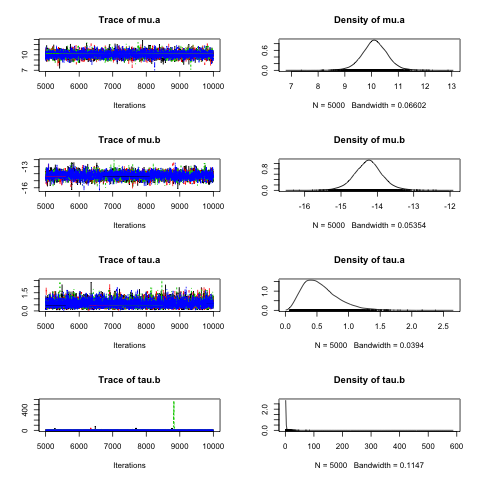
\includegraphics[scale = 0.4]{../JAGSExamples/graphs/hierarchical/linear_plot1.png}
  \end{center}
\end{frame}

\begin{frame}[fragile]
  \begin{verbatim}
Iterations = 5001:10000
Thinning interval = 1 
Number of chains = 4 
Sample size per chain = 5000 

1. Empirical mean and standard deviation for each variable,
   plus standard error of the mean:

          Mean      SD Naive SE Time-series SE
mu.a   10.1173  0.4890 0.003458       0.003566
mu.b  -14.2479  0.3997 0.002826       0.005236
tau.a   0.5579  0.2833 0.002004       0.002953
tau.b   1.8164 10.0432 0.071016       0.350492
  \end{verbatim}
\end{frame}

\begin{frame}[fragile]
  \begin{itemize}
    \item{Let's also implement a hierarchical logit model}
  \end{itemize}
\end{frame}

\begin{frame}[fragile]
  \begin{verbatim}
model
{
  for (i in 1:N)
  {
    y[i] ~ dbern(p[i])
    logit(p[i]) <- a[g[i]] * x[i] + b[g[i]]
  }
  
  for (j in 1:K)
  {
    a[j] ~ dnorm(mu.a, tau.a)
    b[j] ~ dnorm(mu.b, tau.b)
  }
  \end{verbatim}
\end{frame}

\begin{frame}[fragile]
  \begin{verbatim}
  mu.a ~ dnorm(0, 0.0001)
  mu.b ~ dnorm(0, 0.0001)

  tau.a <- pow(sigma.a, -2)
  tau.b <- pow(sigma.b, -2)
  sigma.a ~ dunif(0, 1000)
  sigma.b ~ dunif(0, 1000)
}
  \end{verbatim}
\end{frame}

\begin{frame}[fragile]
  \begin{verbatim}
library('rjags')

df <- read.csv(file.path('data',
                         'hierarchical',
                         'hierarchical_logit.csv'))
  \end{verbatim}
\end{frame}

\begin{frame}[fragile]
  \begin{verbatim}
"g","t","x","y"
1,1,2.01681931037456,1
1,2,9.44675268605351,0
1,3,6.2911404389888,0
...
25,48,6.72132012201473,0
25,49,3.42435503611341,0
25,50,7.37378113903105,0
  \end{verbatim}
\end{frame}

\begin{frame}
  For the sample data:
  \begin{itemize}
    \item{$y \sim f(a_{g(i)} x + b_{g(i)})$}
    \item{$\mu_a = 0.5$}
    \item{$\mu_b = -2$}
  \end{itemize}
\end{frame}

\begin{frame}[fragile]
  \begin{verbatim}
jags <- jags.model(file.path('bugs',
                             'hierarchical',
                             'hierarchical_logit.bugs'),
                   data = list('x' = with(df, x),
                               'y' = with(df, y),
                               'g' = with(df, g),
                               'N' = nrow(df),
                               'K' = with(df, max(g))),
                   n.chains = 4,
                   n.adapt = 5000)

mcmc.samples <- coda.samples(jags,
                             c('mu.a',
                             'mu.b',
                             'tau.a',
                             'tau.b'),
                             5000)

plot(mcmc.samples)

summary(mcmc.samples)
  \end{verbatim}
\end{frame}

\begin{frame}[fragile]
  \begin{center}
    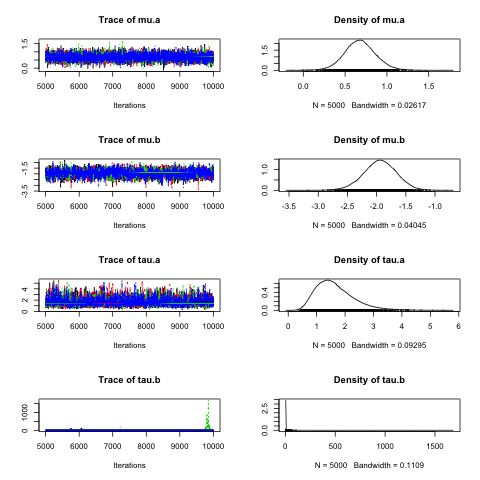
\includegraphics[scale = 0.4]{../JAGSExamples/graphs/hierarchical/logit_plot1.png}
  \end{center}
\end{frame}

\begin{frame}[fragile]
  \begin{verbatim}
Iterations = 5001:10000
Thinning interval = 1 
Number of chains = 4 
Sample size per chain = 5000 

1. Empirical mean and standard deviation for each variable,
   plus standard error of the mean:

         Mean      SD Naive SE Time-series SE
mu.a   0.6795  0.1854 0.001311       0.002471
mu.b  -1.9432  0.2827 0.001999       0.006487
tau.a  1.6534  0.6791 0.004802       0.013086
tau.b  3.8376 31.0577 0.219611       1.581173
  \end{verbatim}
\end{frame}

\begin{frame}[fragile]
  \begin{itemize}
    \item{Both of these hierarchical models are very powerful in practice}
    \item{Try them out on your data and see if they make better predictions on held out data}
  \end{itemize}
\end{frame}

\begin{frame}[fragile]
  \begin{itemize}
    \item{As one of two closing models, let's implement the ideal points model}
    \item{This model is quite complex to implement without Bayesian methods}
    \item{It also produces beautiful results}
  \end{itemize}
\end{frame}

\begin{frame}[fragile]
  \begin{verbatim}
Senator,Bill,Vote
BYRD (D WV),2,0
ENZI (R WY),2,1
  \end{verbatim}
\end{frame}

\begin{frame}[fragile]
  \begin{verbatim}
model
{
  for (i in 1:M)
  {
    for (j in 1:N)
    {
      votes[i, j] ~ dbern(p[i, j])
      logit(p[i, j]) <- g[j] * (a[i] - b[j])
    }
  }
  \end{verbatim}
\end{frame}

\begin{frame}[fragile]
  \begin{verbatim}
  for (i in 1:M)
  {
    a[i] ~ dnorm(0, tau.a)
  }

  tau.a <- pow(sigma.a, -2)
  sigma.a ~ dunif(0, 100)
  \end{verbatim}
\end{frame}

\begin{frame}[fragile]
  \begin{verbatim}
  for (j in 1:N)
  {
    b[j] ~ dnorm(mu.b, tau.b)
    g[j] ~ dnorm(0, tau.g)
   }

  mu.b ~ dnorm(0, .0001)

  tau.b <- pow(sigma.b, -2)
  sigma.b ~ dunif(0, 100)

  tau.g <- pow(sigma.g, -2)
  sigma.g ~ dunif(0, 100)
}
  \end{verbatim}
\end{frame}

\begin{frame}[fragile]
  \begin{verbatim}
library('rjags')

binary.votes <- read.table(file.path('data',
                                     'ideal_points',
                                     'ideal_points.txt'))
binary.votes <- as.matrix(binary.votes)
  \end{verbatim}
\end{frame}

\begin{frame}[fragile]
  \begin{verbatim}
a <- rep(NA, nrow(binary.votes))
a[which(row.names(binary.votes) == "COBURN (R OK)")] <- 2

jags <- jags.model(file.path('bugs',
                             'ideal_points',
                             'ideal_points.bugs'),
                   data = list('votes' = binary.votes,
                               'M' = nrow(binary.votes),
                               'N' = ncol(binary.votes),
                               'a' = a),
                   n.chains = 4,
                   n.adapt = 500)
  \end{verbatim}
\end{frame}

\begin{frame}[fragile]
  \begin{verbatim}
j.samples <- jags.samples(jags,
                        c('a', 'b', 'g'),
                        250)

estimated.a <- apply(j.samples$a, 1, mean)

df <- data.frame(Senator = row.names(binary.votes),
                 IdealPoint = estimated.a)
head(df)
tail(df)
  \end{verbatim}
\end{frame}

\begin{frame}[fragile]
  \begin{verbatim}
           Senator IdealPoint
1     BUSH (R USA)   1.321483
2  SESSIONS (R AL)   2.042710
3    SHELBY (R AL)   1.346424
4 MURKOWSKI (R AK)   1.000675
5   STEVENS (R AK)   1.069571
6       KYL (R AZ)   1.757788
               Senator IdealPoint
97         BYRD (D WV) -0.7941595
98  ROCKEFELLER (D WV) -1.1672899
99     FEINGOLD (D WI) -1.5509000
100        KOHL (D WI) -1.0407957
101        ENZI (R WY)  1.8374551
102      THOMAS (R WY)  1.8247487
  \end{verbatim}
\end{frame}

\begin{frame}[fragile]
  \begin{itemize}
    \item{As a last model, we'll implement a mixture of two Gaussians}
  \end{itemize}
\end{frame}

\begin{frame}[fragile]
  \begin{verbatim}
model
{
  for (i in 1:N)
  {
    z[i] ~ dbern(p)
    mu[i] <- z[i] * mu1 + (1 - z[i]) * mu2
    x[i] ~ dnorm(mu[i], tau)
  }
  
  p ~ dbeta(1, 1)
  
  mu1 ~ dnorm(0, 0.0001)
  mu2 ~ dnorm(1, 0.0001)
  
  tau <- pow(sigma, -2)
  sigma ~ dunif(0, 100)
}
  \end{verbatim}
\end{frame}

\begin{frame}[fragile]
  \begin{verbatim}
library('rjags')

df <- read.csv(file.path('data',
                         'mixture_models',
                         'two_normals.csv'))
  \end{verbatim}
\end{frame}

\begin{frame}[fragile]
  \begin{center}
    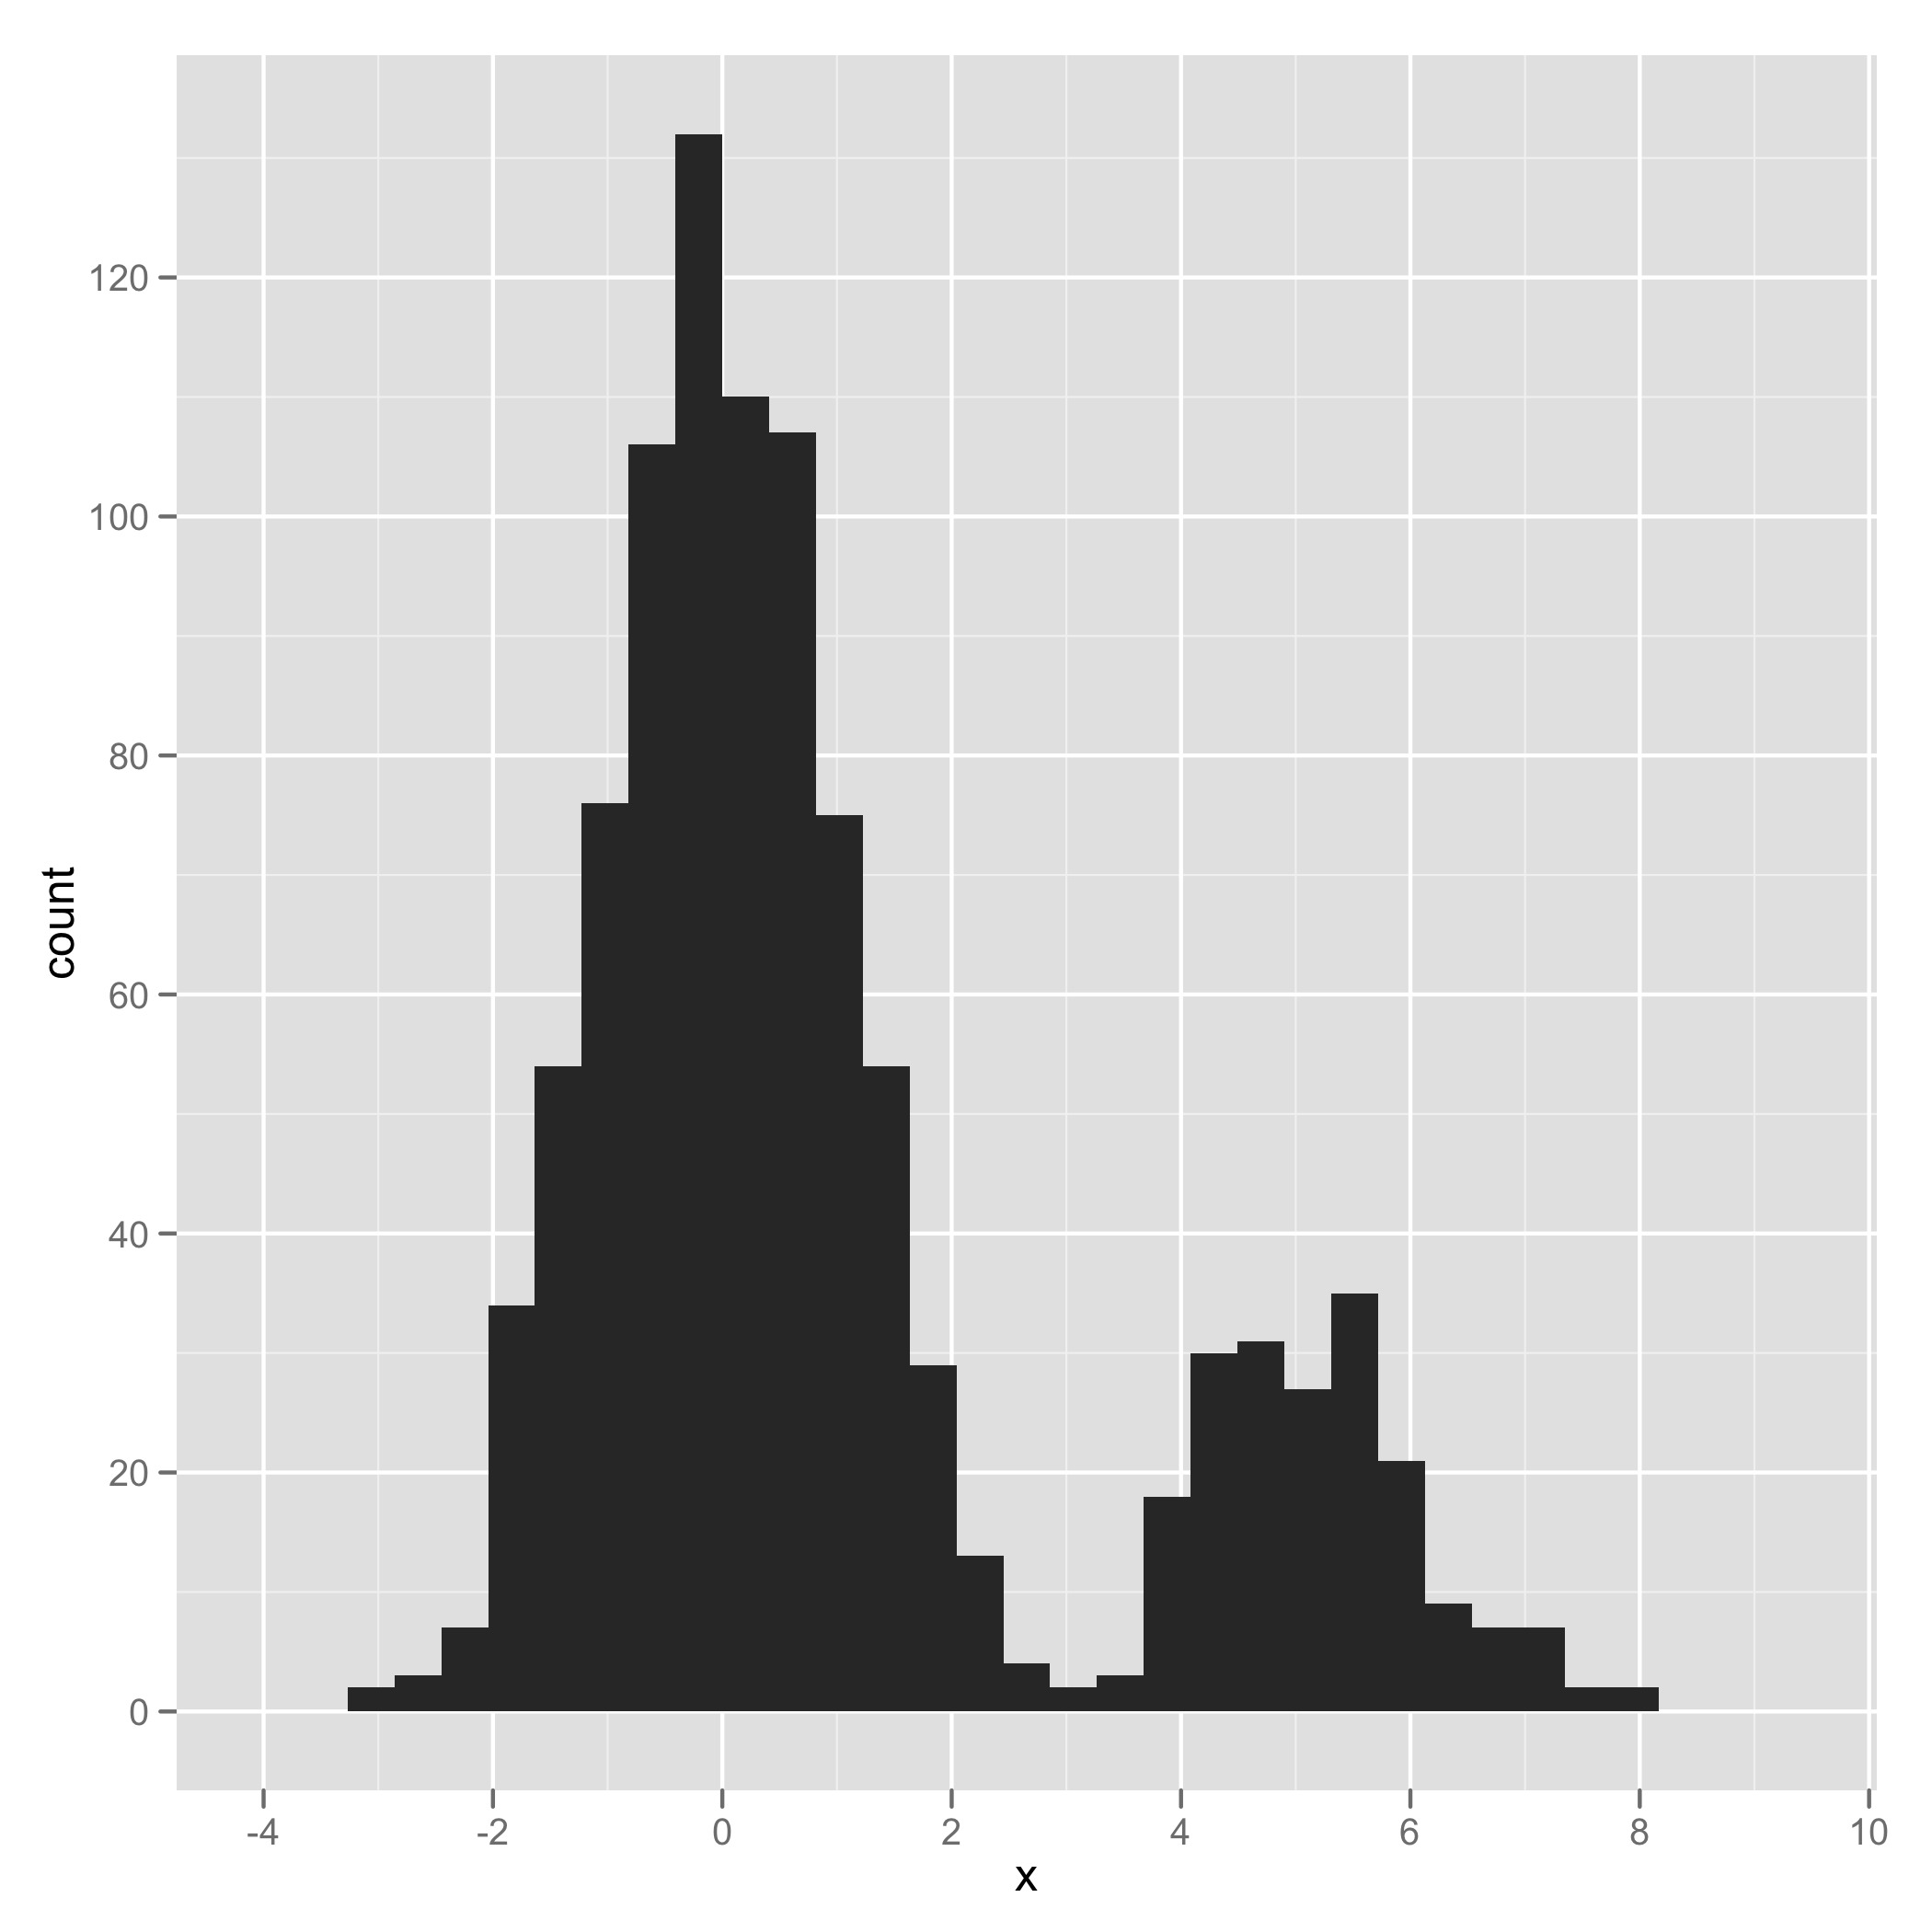
\includegraphics[scale = 0.1]{../JAGSExamples/graphs/mixture_models/blind_histogram.png}
  \end{center}
\end{frame}

\begin{frame}[fragile]
  \begin{center}
    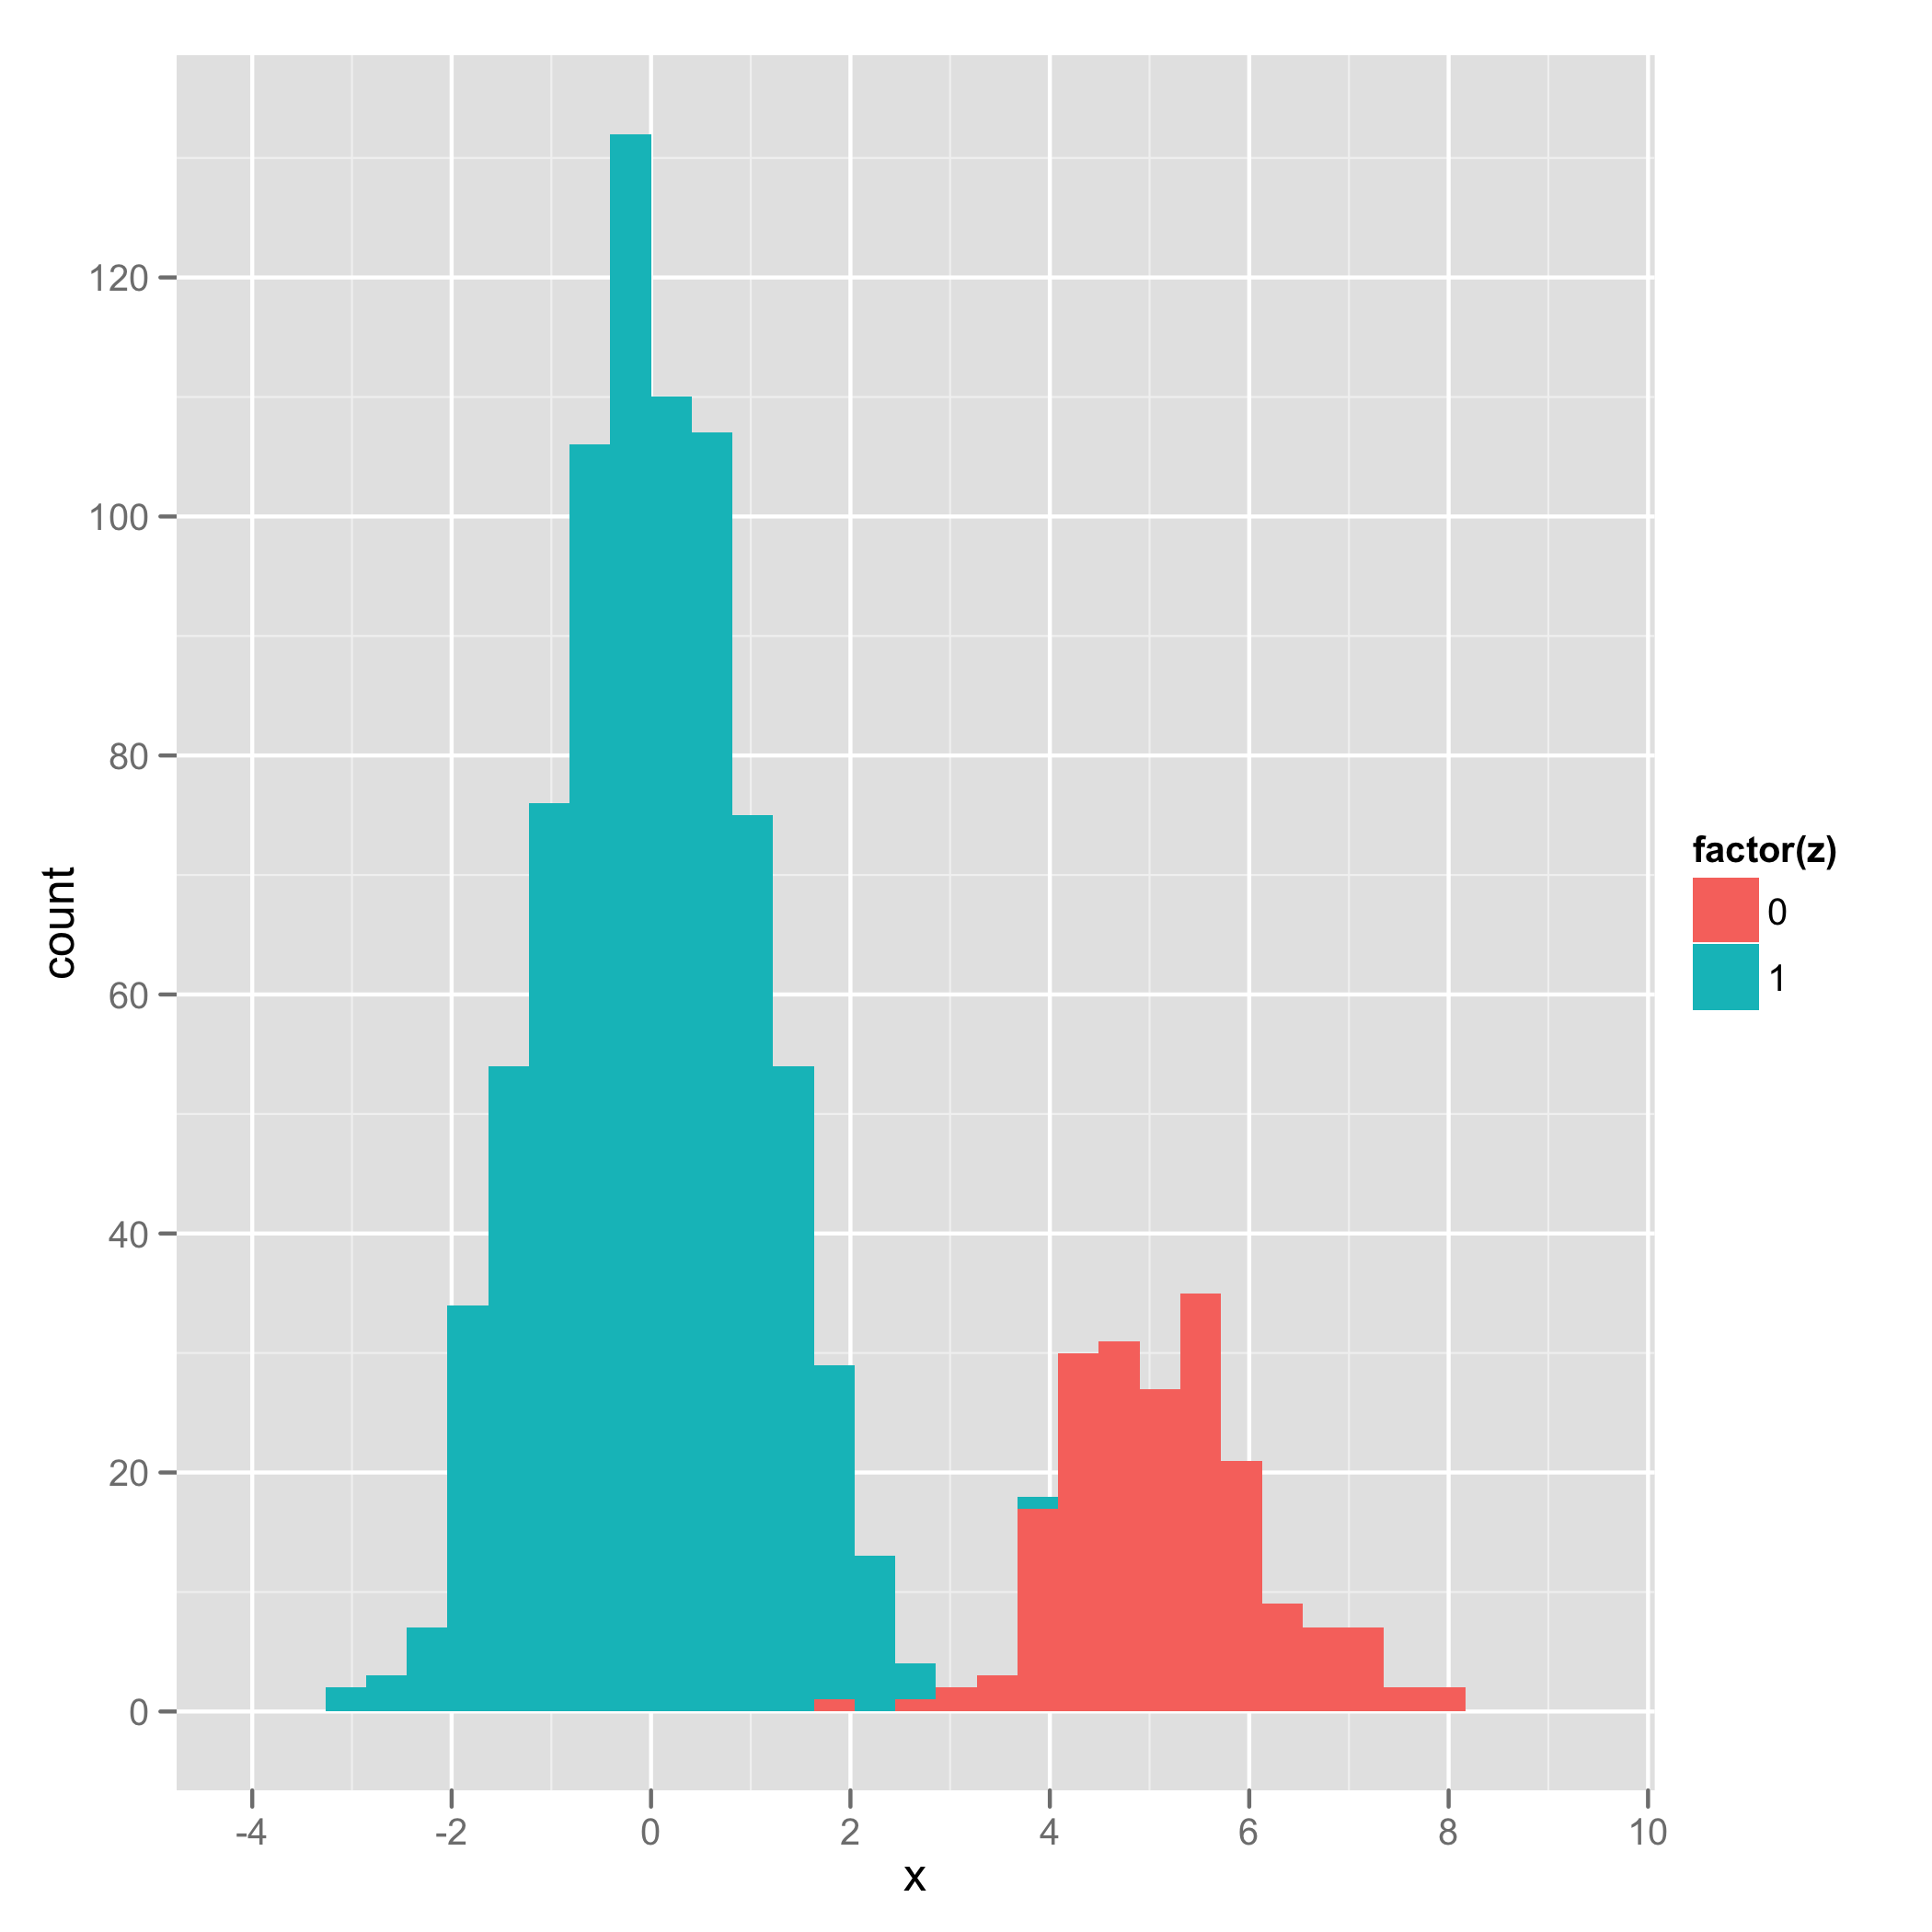
\includegraphics[scale = 0.1]{../JAGSExamples/graphs/mixture_models/labelled_histogram.png}
  \end{center}
\end{frame}

\begin{frame}[fragile]
For the sample data:
  \begin{itemize}
    \item{$p = 0.8$}
    \item{$\mu_1 = 0$}
    \item{$\mu_2 = 5$}
    \item{$\sigma = 1$}
  \end{itemize}
\end{frame}

\begin{frame}[fragile]
  \begin{verbatim}
jags <- jags.model(file.path('bugs',
                             'mixture_models',
                             'two_normals.bugs'),
                   data = list('x' = with(df, x),
                               'N' = nrow(df)),
                   n.chains = 4,
                   n.adapt = 1000)
 
mcmc.samples <- coda.samples(jags,
                             c('p', 'mu1', 'mu2', 'sigma'),
                             5000)

plot(mcmc.samples)

summary(mcmc.samples)
  \end{verbatim}
\end{frame}

\begin{frame}[fragile]
  \begin{center}
    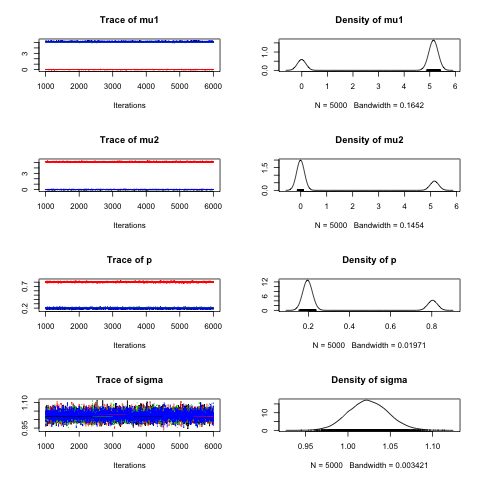
\includegraphics[scale = 0.4]{../JAGSExamples/graphs/mixture_models/two_normals_plot1.png}
  \end{center}
\end{frame}

\begin{frame}[fragile]
  \begin{verbatim}
Iterations = 1001:6000
Thinning interval = 1 
Number of chains = 4 
Sample size per chain = 5000 

1. Empirical mean and standard deviation for each variable,
   plus standard error of the mean:

       Mean      SD  Naive SE Time-series SE
mu1   3.858 2.23225 0.0157844      5.426e-04
mu2   1.281 2.23140 0.0157784      3.988e-04
p     0.348 0.26360 0.0018640      8.817e-05
sigma 1.024 0.02339 0.0001654      2.155e-04
  \end{verbatim}
\end{frame}

\begin{frame}
  \begin{itemize}
    \item{We'll stop there, but BUGS can easily be used for other models:}
    \begin{itemize}
      \item{LDA with a fixed number of topics}
      \item{Social Network Analysis via the stochastic blockmodel}
      \item{$\ldots$}
    \end{itemize}
  \end{itemize}
\end{frame}

\end{document}
